\documentclass[11pt,french]{article}

\usepackage[utf8]{inputenc}
\usepackage[T1]{fontenc}
\usepackage{amsmath}
\usepackage{textcomp}


\usepackage{graphicx}


\usepackage{geometry}
\geometry{letterpaper, margin=1in}

\usepackage{url}
\usepackage{caption}
\newcommand{\source}[1]{\caption*{Source: {#1}} }

\begin{document}

\thispagestyle{empty}

\begin{center}

\vspace{3cm}

{ \LARGE \bfseries Chapitre 5 \\ }
Cours : Mathématiques financières \\

\vfill

\textsc{École d'actuariat}\\
Université Laval\\
Automne 2019

\end{center}

\newpage

\section {Question 1}
\subsection{a)}
On a la figure suivante : 

\begin{figure}[h!] % h = here pour ici, b = bottom pour bas de page, t = top pour haut de page
    \centering
    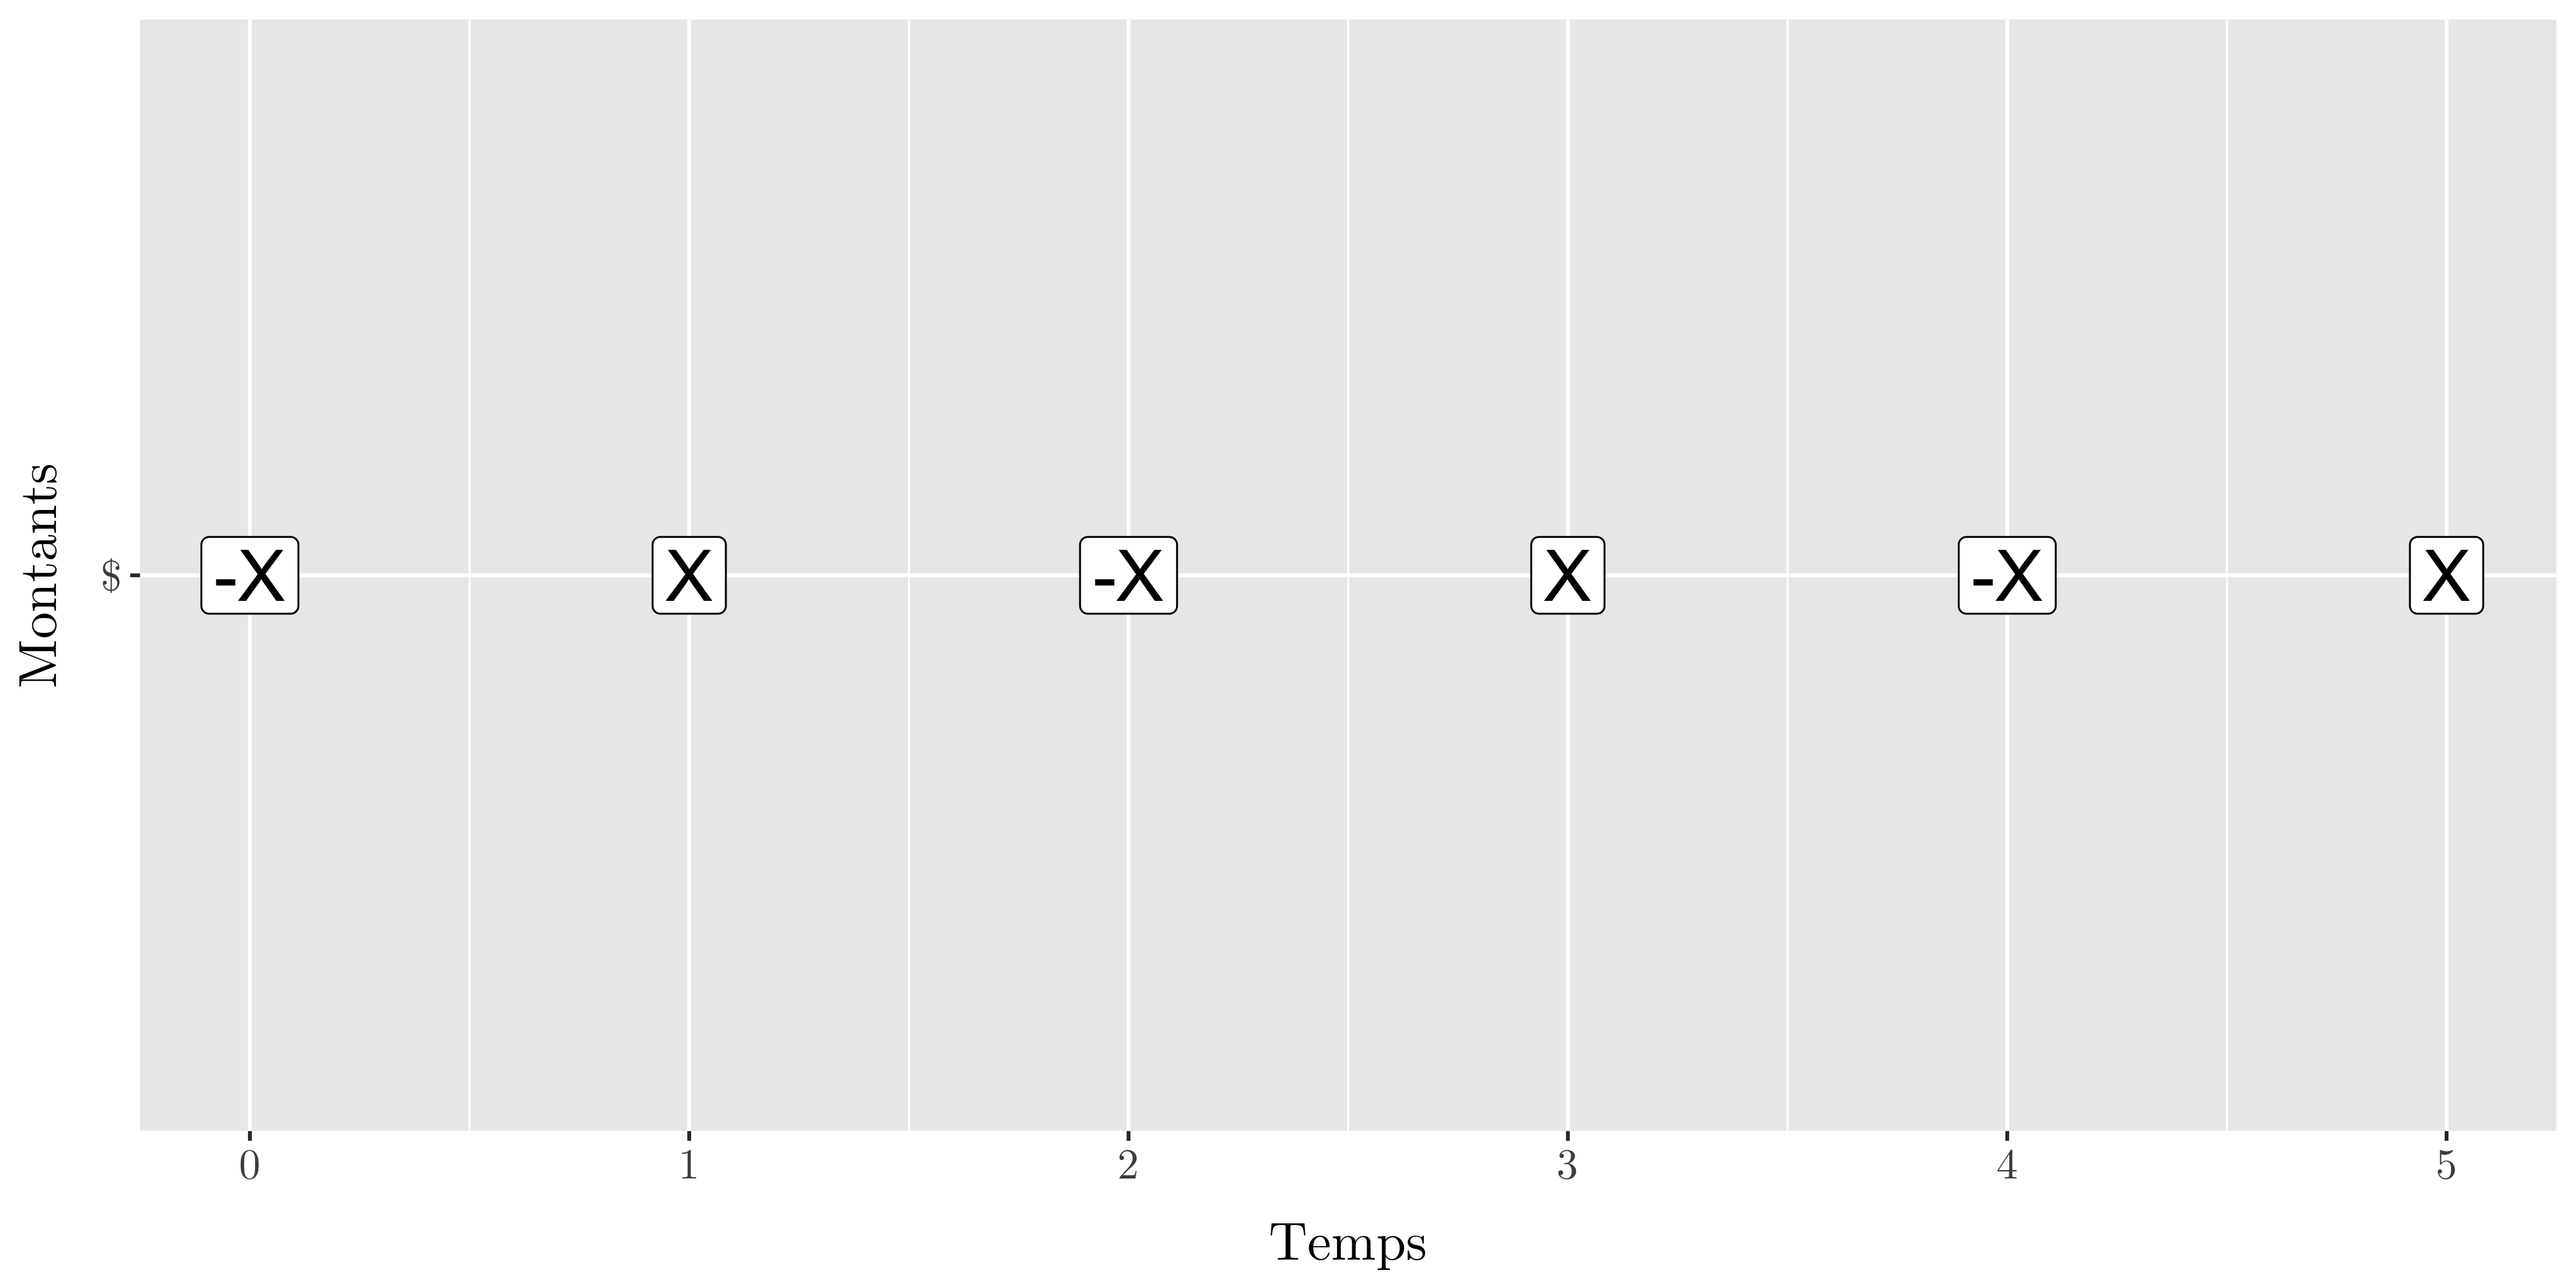
\includegraphics[width=1\textwidth]{Figures/figure1.png}
\end{figure}

L'équation à résoudre est donc la suivante
$$
-X + Xv - Xv^2 + Xv^3 - Xv^4 + Xv^5 = Xv^6
$$
$$
-1 + v - v^2 + v^3 - v^4 + v^5 = v^6
$$
$$
-1 + v - v^2 + v^3 - v^4 + v^5 - v^6 = 0
$$

\subsection{b)}
Thomas ne demande jamais d'utiliser la BA2+. On peut cependant tester un taux quelconque, disons 20 \%.

$$
-1 + v - v^2 + v^3 - v^4 + v^5 - v^6 = -0.697 680
$$

Ainsi, 20\% n'est pas le bon taux, mais il est très proche du taux cherché. En utilisant un solveur (comme celui de Excel ou de la BA2+), on obtient un TRI d'environ 19\%.

\section{Question 2}
\begin{figure}[h!] % h = here pour ici, b = bottom pour bas de page, t = top pour haut de page
    \centering
    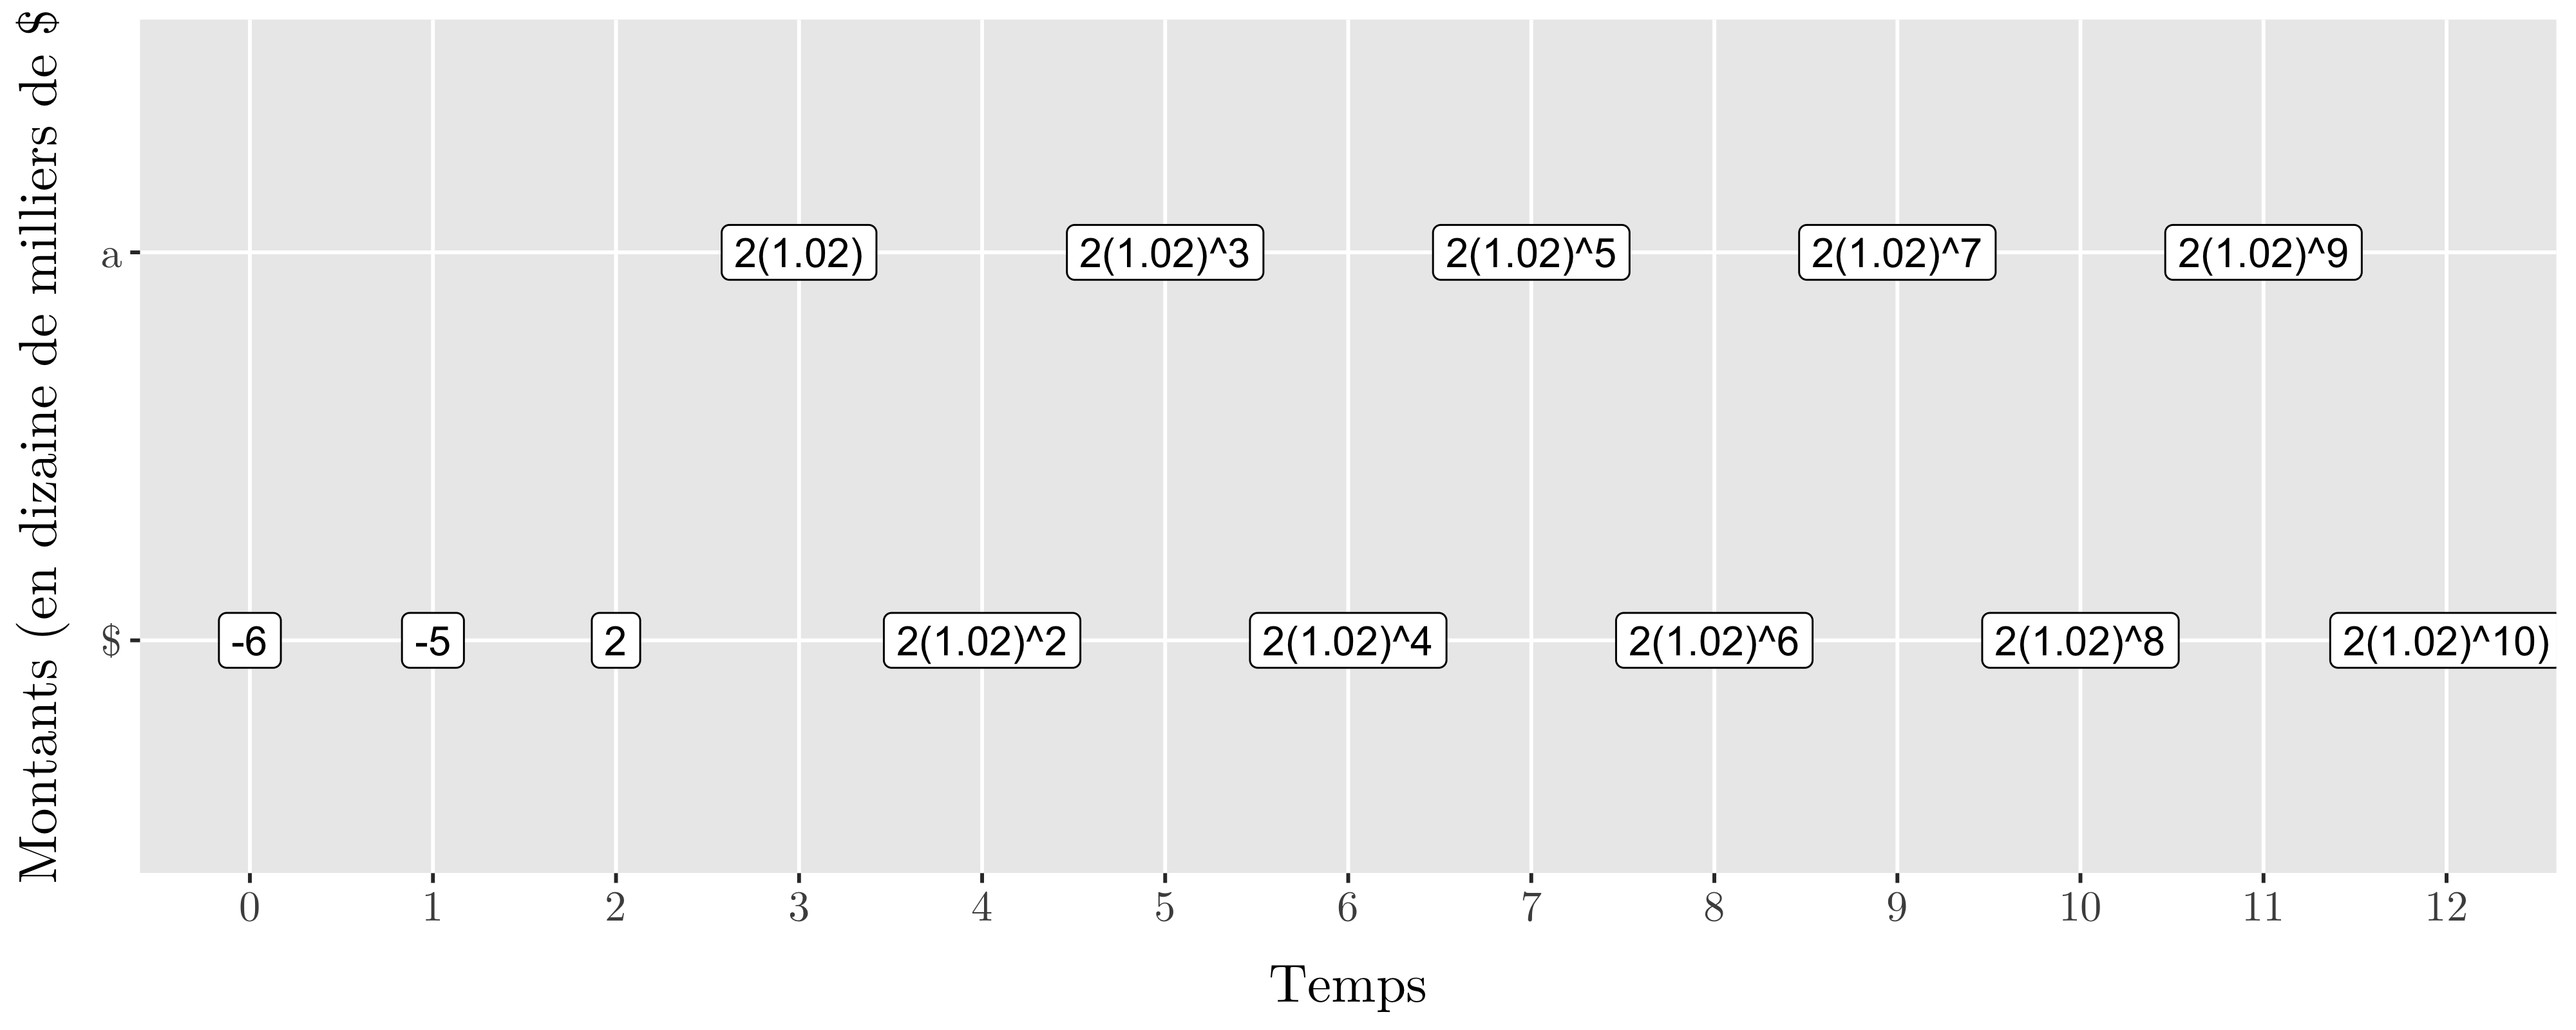
\includegraphics[width=1\textwidth]{Figures/figure2.png}
\end{figure}

L'équation à résoudre est la suivante :
$$
VAN = -60K -50Kv + v^2 [20K + 20K(1.02)v + 20K(1.02)^2v^2 + … + 20K(1.02)^{10}Kv^{10}]
$$
$$
VAN = -60K -50Kv + 20Kv^2 [1 + (1.02)v +(1.02)^2v^2 + … + (1.02)^{10}Kv^{10}]
$$
$$
VAN = -60K -50Kv + 20Kv^2 \sum_{i=0}^9 1.02v^k
$$
$$
VAN = -60K -50Kv + 20Kv^2 \left( \frac{1 - (1.02v)^{10}}{1 - 1.02v} \right)
$$
$$
VAN = 3842.218
$$

\section{Question 3}
\begin{figure}[h!] % h = here pour ici, b = bottom pour bas de page, t = top pour haut de page
    \centering
    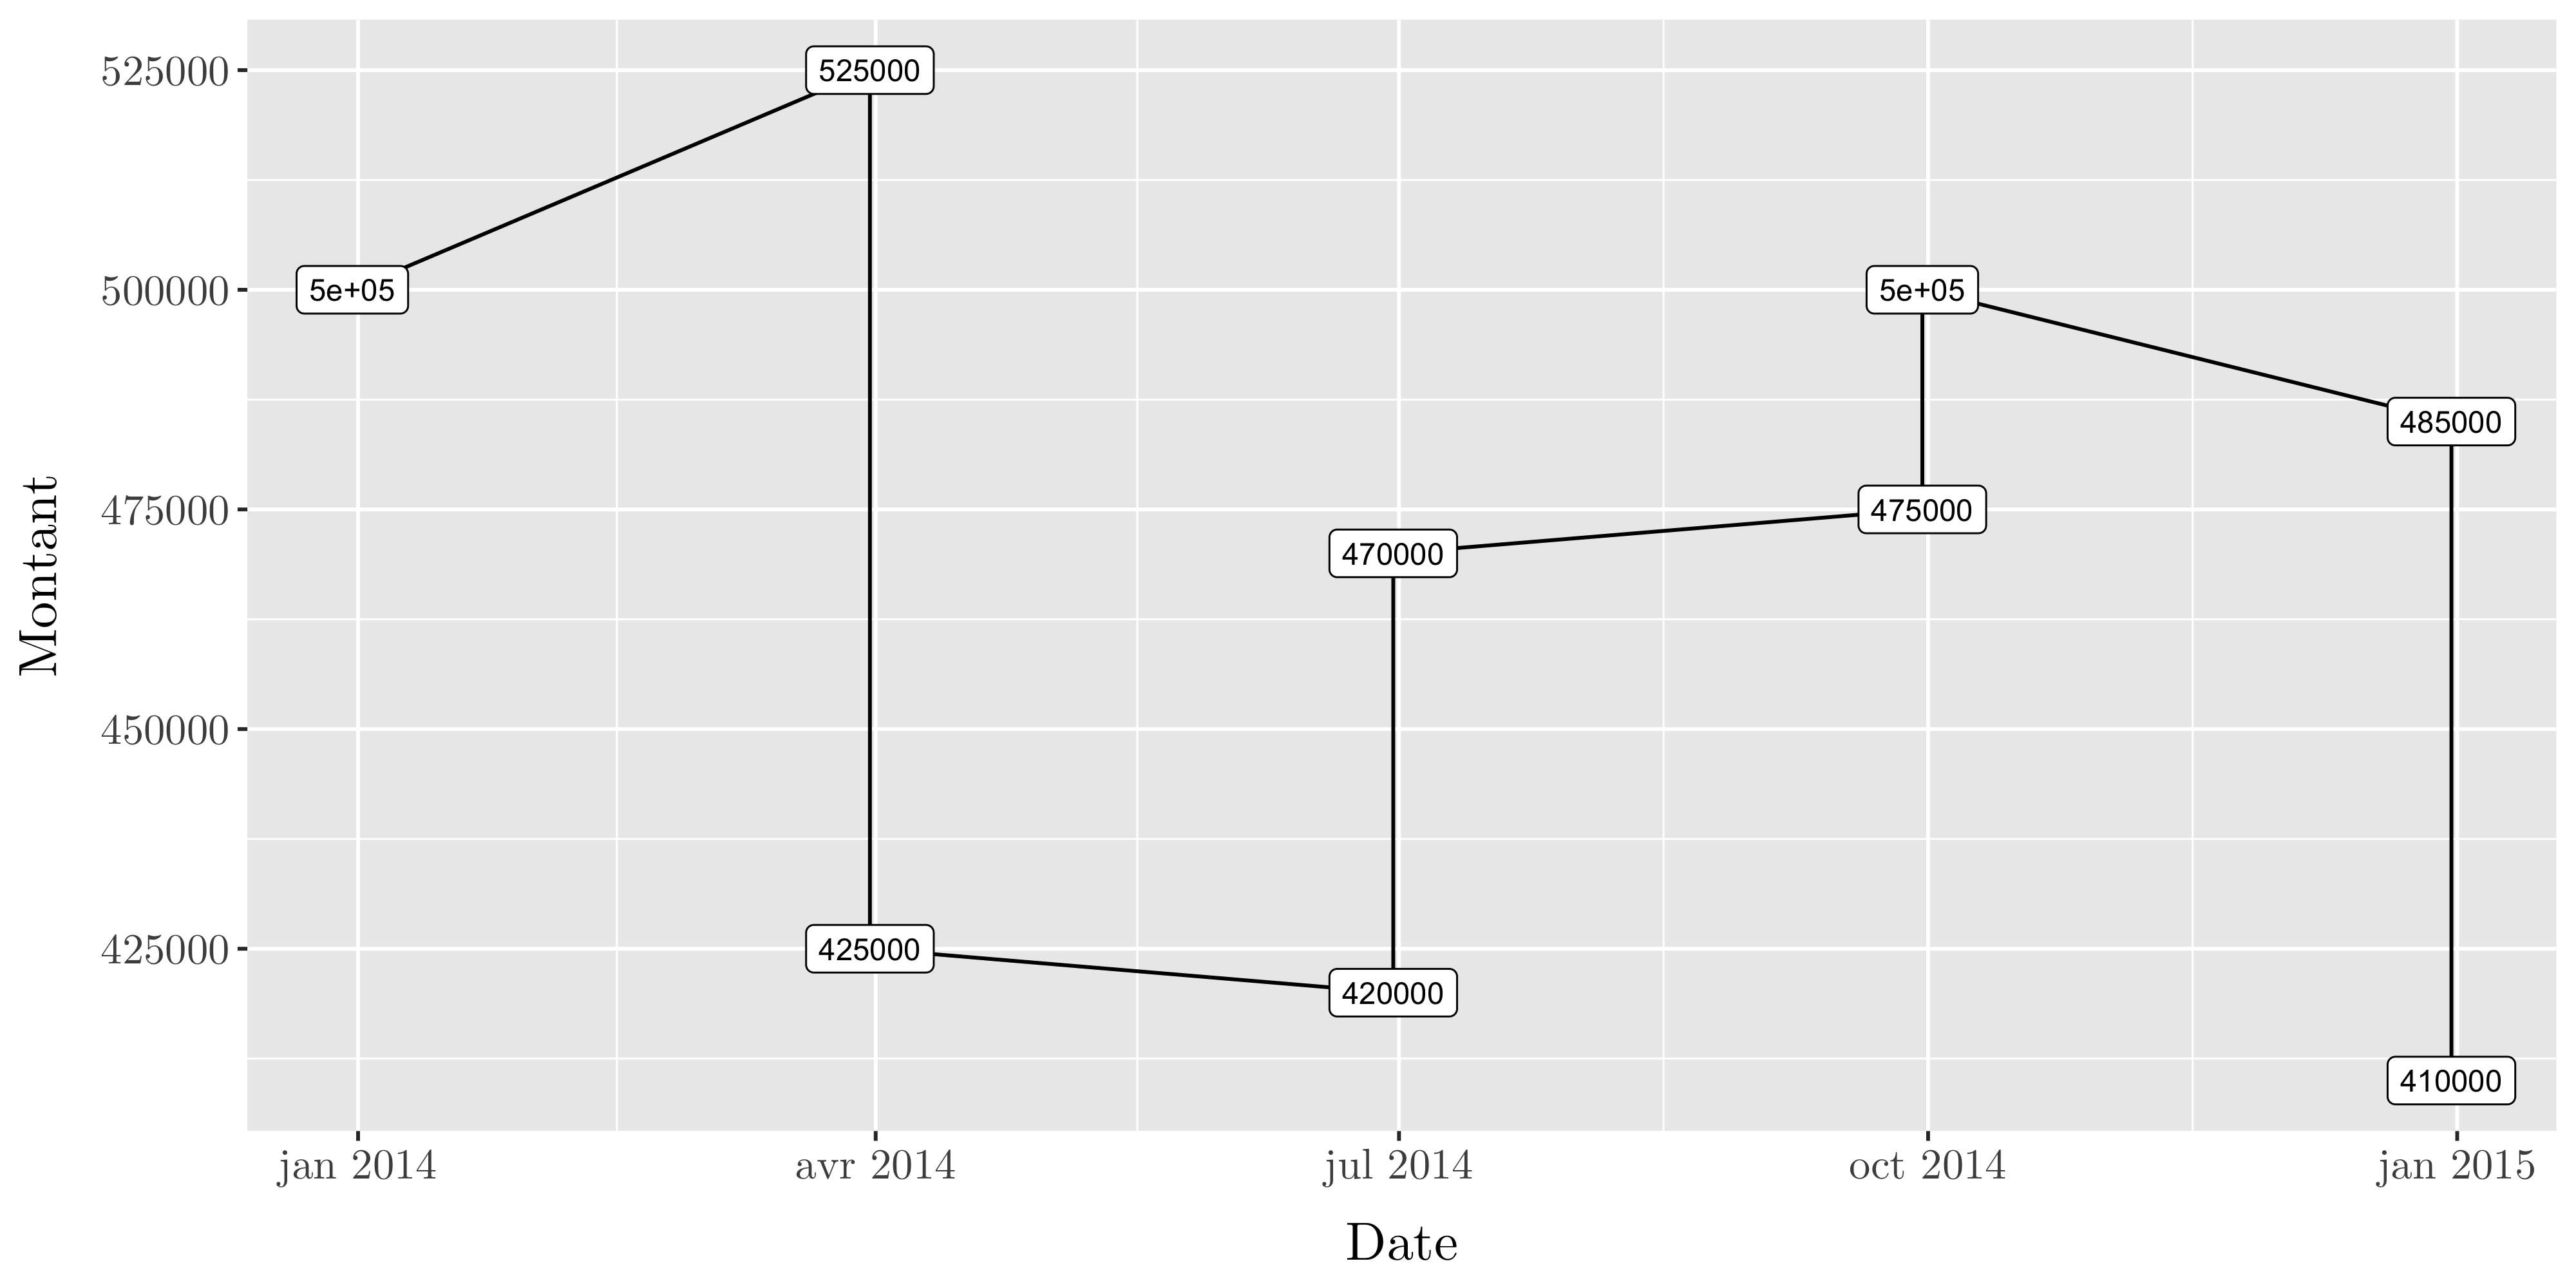
\includegraphics[width=1\textwidth]{Figures/figure3.png}
\end{figure}

\subsection{a}
La logique est toujours la même. Au numérateur, on a la valeur finale moins la somme de tous les retraits et les dépôts au courant de l'année et au dénominateur, on a les valeurs de tous les dépôts et les retraits multipliées par la fraction de l'année durant laquelle elles ces dernières ont respectivement pu créer du rendement. On a $C_i$, la valeur du retrait ou du dépôt à $t_i$, $n$, le nombre de dépôts et $v_f$, la valeur finale dans le compte. 

On a donc 
$$
I = \frac{v_f - \sum_{i=1}^n C_i}{\sum_{i=1}^n (1 - t_i) \times C_i}
$$

$$
I = \frac{410000 - (500000 - 100000 + 50000 + 25000 - 75000)}
{500000 - 100000 (1 - 0.25) + 50000 (1 - 0.5) + 25000 ( 1 - 0.75) - 75000 (1-1)}
$$
$$
I = \frac{10000}{456250}
$$

\subsection{b}
On a l'équation suivante :
$$
\left(\frac{525000}{500000}\times \frac{420000}{425000}
\times \frac{475000}{470000}\times\frac{485000}{500000} \right) - 1
$$

\section{Question 4}
On a la relation suivante :
$$
1 \$ \times (1.07) \times (1.06) = 1.1342 \$
$$
\end{document}

